\documentclass[11pt]{article}
\usepackage[utf8]{inputenc} % Para caracteres en espa�ol
\usepackage{amsmath,amsthm,amsfonts,amssymb,amscd}
\usepackage{multirow,booktabs}
\usepackage[table]{xcolor}
\usepackage{fullpage}
\usepackage{lastpage}
\usepackage{enumitem}
\usepackage{multicol}
\usepackage{fancyhdr}
\usepackage{mathrsfs}
\usepackage{pdfpages}
\usepackage{wrapfig}
\usepackage{setspace}
\usepackage{esvect}
\usepackage{calc}
\usepackage{multicol}
\usepackage{cancel}
\usepackage{graphicx}
\graphicspath{ {pictures/} }
\usepackage[retainorgcmds]{IEEEtrantools}
\usepackage[margin=3cm]{geometry}
\usepackage{amsmath}
\newlength{\tabcont}
\setlength{\parindent}{0.0in}
\setlength{\parskip}{0.05in}
\usepackage{empheq}
\usepackage{framed}
\usepackage[most]{tcolorbox}
\usepackage{xcolor}
\colorlet{shadecolor}{orange!15}
\parindent 0in
\parskip 12pt
\geometry{margin=1in, headsep=0.25in}
\theoremstyle{definition}
\newtheorem{defn}{Definition}
\newtheorem{reg}{Rule}
\newtheorem{exer}{Exercise}

% Two more packages that make it easy to show MATLAB code
\usepackage[T1]{fontenc}
\usepackage[framed,numbered]{matlab-prettifier}
\lstset{
	style = Matlab-editor,
	basicstyle=\mlttfamily\small,
}

\newtheorem{note}{Note}
\begin{document}
\setcounter{section}{0}

\thispagestyle{empty}

\begin{center}
{\LARGE \bf Homework 3 Problem 5}\\
{\large AE403 - Spring 2018 \\ Emilio R. Gordon}
\end{center}
\vspace{20mm}
For Homework 3 Problem 5 we are tasked with designing and simulating a spin-up maneuver for a space-craft that is not axis-symmetric. In particular, consider a satellite with the principle moments of inertia:
\begin{equation*}
\begin{aligned}
J^2 = 
\begin{bmatrix}
4600 & 0 & 0 \\ 0 & 4400 & 0 \\ 0 & 0 & 750
\end{bmatrix}
[kg \cdot m^2]
\end{aligned}
\end{equation*}

The goal is to achieve a spin rate of 60 rpm or 1 revolution per second about the minor axis $\hat{z}$ Spin thruster are available that exert a constant torque about  $\hat{z}$ of $\tau_z = 100 N\cdot m$. The satellite begins with an angular velocity of $\omega = 0.0001 \hat{x}$. Note: Given these $J$, we can assume our craft to have a "soup can", prolate shape since $J_t > J_a$.

{\Large\textbf{Part A}}

Part A requires us to assume that the craft is axis-symmetric such that $J_1 = J_2 = 4500 \, [kg \cdot m^2]$. We are tasked with finding the duration of time for which the spin thrusters should be fired for in order to reach the desired spin rate of 60rpm about the minor z-axis.

To accomplish this we must recall what the case for "spin-up" motion entailed. Assuming a constant torque applied in the z-direction and axis-symmetric geometry, our Euler's Equations reduce to:

\begin{equation*}
\begin{aligned}
\left\{\begin{matrix}
0 = J_t \, \dot{\omega_x} - (J_t-J_a)\omega_y\omega_z\\ 
0 = J_t \, \dot{\omega_y} + (J_t-J_a)\omega_x\omega_z\\ 
\tau_z = J_a\, \dot{\omega_z}
\end{matrix}\right.
\end{aligned}
\end{equation*}
Allowing us to derive
\begin{equation*}
\begin{aligned}
\tau_z &= J_a\, \dot{\omega_z} \\
&\rightarrow  \dot{\omega_z} = \frac{\tau_z}{J_a} \\
&\Rightarrow \omega_z = \frac{\tau_z}{J_a}\,t + \omega_z(0)
\end{aligned}
\end{equation*}

Recall that our $\omega_z(0) = 0$. Solving for time gives us:
\begin{equation*}
\begin{aligned}
t = \frac{\omega \, J_a}{\tau_z}
\end{aligned}
\end{equation*}

Which when plugging in: $J_a= 750 \, [kg \cdot m^2]$, $\tau_z = 00 \, [\frac{kg \,m^3}{s^2}]$, $\omega_z = 1 \, [\frac{\text{revolution}}{\text{second}}]$...

We arrive at \textbf{t = 7.5 seconds}.
\newpage
{\Large\textbf{Part B}}

To animate this, we must establish the following initial conditions. The problem states that the craft is in the orientation of the body frame with respect to the base frame and $\omega$ written in the body fixed coordinates. In addition, the body is initially aligned with the base frame meaning we can used the identity matrix for $R$.

The code of such is:
\begin{figure}[h!]
\begin{lstlisting}
J1 = 4600; % kgm^3
J2 = 4400; % kgm^3
J3 = 750;  % kgm^3
R0 = eye(3);
w0 = [1e-1; 0; 0];
J = [J1 0 0; 0 J2 0; 0 0 J3];
tMax = 7.5;
\end{lstlisting}
\caption{Initial Conditions}
\end{figure}

Now we must write functions for computing $\dot{\omega}$ and $\dot{R}$. This can easily be done by simultaneously integrating Euler's Equations to find the angular velocity and using the relation $\dot{R} = R \hat{\omega}$ to find the rotation matrix change with respect to time. This is accomplished in the function xdot shown in Figure 2 below.
\begin{figure}[h!]
\begin{lstlisting}
function xdot = f(t,x,J)
R = XtoR(x(1:9,1))
w = x(10:end,1)
zTorque = 100;
%CODE TO COMPUTE Rdot and wdot
w1 = w(1);
w2 = w(2);
w3 = w(3);
what = [0 -w3 w2; w3 0 -w1; -w2 w1 0];

Rdot = R*what;

wd1 = ((J(2,2)-J(3,3))/(J(1,1)))*w3*w2;
wd2 = ((J(3,3)-J(1,1))/(J(2,2)))*w3*w1;
wd3 = (zTorque + (J(1,1)-J(2,2))*w1*w2)/J(3,3);

wdot = [wd1;wd2;wd3];

xdot = [RtoX(Rdot); wdot];
\end{lstlisting}
\caption{Functions Rates of Change}
\end{figure}

From part a, we discovered that in order to achieve a spin-rate of 1 revolution per second, the thruster must be powered on for 7.5 seconds. By taking the last entries of the x varialbe produced by the ODE we can get the final states for the rotation matrix and angular velocity. Note however, that 7.5 seconds was the result for the case where the satellite was axis-symmetric. In this problem, the satellite is almost axis-symmetric but not quite. We find that the actual spin-up time to reach a spin-rate of 1 revolution per second is 7.578 seconds. Doing so results in...
\begin{equation*}
\begin{aligned}
R = \begin{bmatrix}
-0.7734  &  0.6338  &  0.0002 \\
   -0.6338 &  -0.7734  & -0.0007 \\
   -0.0003 &  -0.0007 &   1.0000 \\
\end{bmatrix} \qquad \qquad \omega = \begin{bmatrix}
-0.0001 \\
    0.0000 \\
    1.0000 \\
\end{bmatrix}
\end{aligned}
\end{equation*}

To better illustrate this, the code can be modified to "turn-off" the thruster after this time. The benefit of this would allow us to observe the motion and behavior of the satellite once it has reached a spin-rate of 1 revolution per minute about the z axis. This was accomplished in figure 3 below.

\begin{figure}[h!]
\begin{lstlisting}
function xdot = f(t,x,J)
R = XtoR(x(1:9,1));
w = x(10:end,1);
zTorque = 100;

w1 = w(1);
w2 = w(2);
w3 = w(3);
what = [0 -w3 w2; w3 0 -w1; -w2 w1 0];

Rdot = R*what;

if t<7.578
    wd1 = ((J(2,2)-J(3,3))/(J(1,1)))*w3*w2;
    wd2 = ((J(3,3)-J(1,1))/(J(2,2)))*w3*w1;
    wd3 = (zTorque + (J(1,1)-J(2,2))*w1*w2)/J(3,3);
else
    wd1 = ((J(2,2)-J(3,3))/(J(1,1)))*w3*w2;
    wd2 = ((J(3,3)-J(1,1))/(J(2,2)))*w3*w1;
    wd3 = ((J(1,1)-J(2,2))*w1*w2)/J(3,3);
end

wdot = [wd1;wd2;wd3];

xdot = [RtoX(Rdot); wdot];\end{lstlisting}
\caption{Functions Rates of Change with "Turn-Off"}
\end{figure}
The results can be shown in the plots below. In this scenario, the simulation runs for 20 seconds but the thruster is cut-off after the aforementioned time.
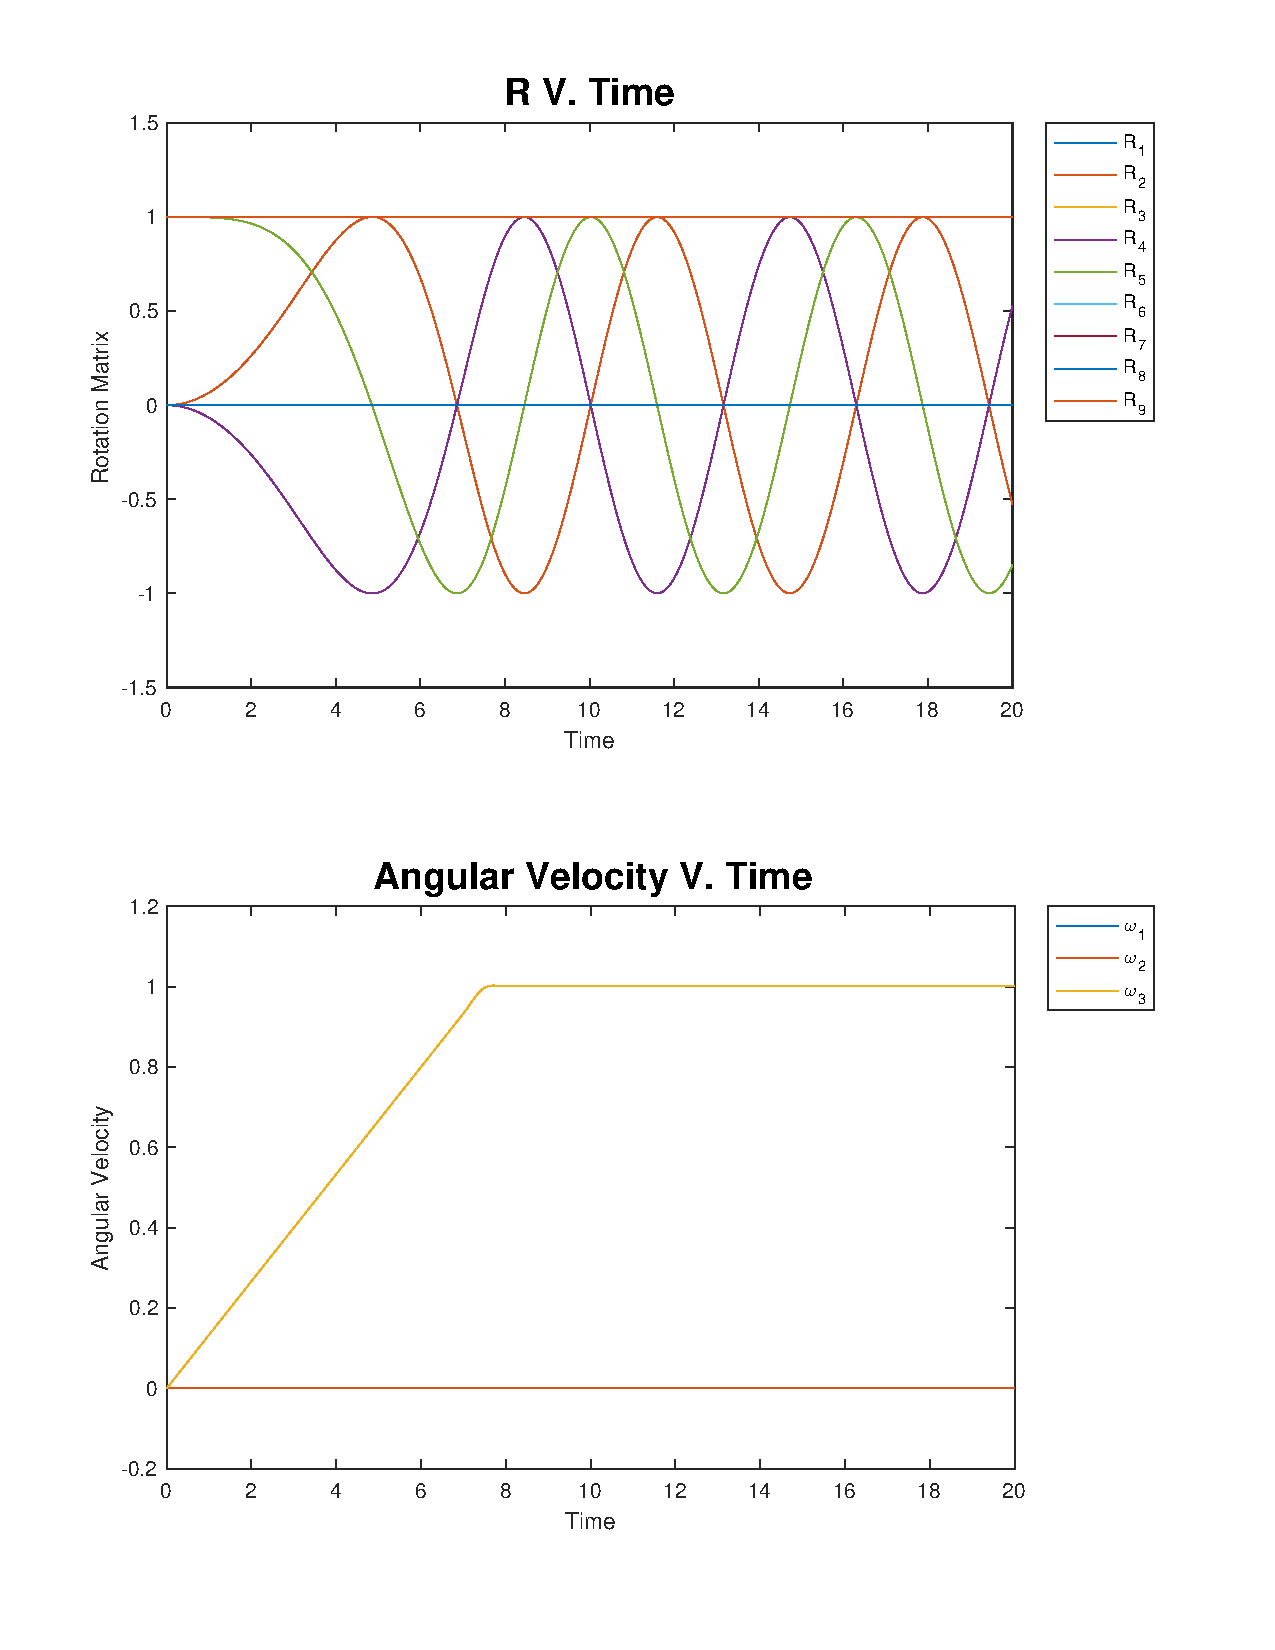
\includepdf{plots.pdf}
\newpage
{\Large\textbf{Part C}}

Part C ask us to repeat the objectives from part b however, now the craft will have larger initial angular velocities in the x-direction. Part B considered an initial angular velocity of 0.0001 (1e-4) in the x-direction. We will no consider initial angular velocities of $\omega_x = 1e-3$, $\omega_x = 1e-2$, $\omega_x = 1e-1$ and $\omega_x = 1$ and observe the resulting effects. 

From watching the simulations, it is clear that for larger values of $\omega_1(0)$ the angular velocity and angular moment struggle to remain constant. We can get a more clear image of what is going on however by looking at the plots. The following pages are the plots for $\omega_x = 1e-4$, $\omega_x = 1e-3$, $\omega_x = 1e-2$, $\omega_x = 1e-1$ and $\omega_x = 1$ respectively. 

Before we begin our study into the angular velocity and angular momentum of the craft with varying initial angular velocities, it is important to remember that the magnitude of angular momentum is fixed and constant.

We can clearly see that in a simulation lasting 20 seconds with a thruster shutdown at 7.5seconds,
\begin{itemize}
\item $\bf{\omega_x = 1e-4}$: This was the original case. We see that   We also see that the angular momentum stays constant in each of the elements.
\begin{itemize} 
\item \textbf{Angular Velocity: }After the engine cutoff, the angular velocities in the y and z are fairly constant and resistant to any major changes.
\item \textbf{Angular Momentum: } After the engine cutoff, the angular momentum elements remain constant, only having influence in the z-direction. 
\end{itemize}
\item $\bf{\omega_x = 1e-3}$:
\begin{itemize} 
\item \textbf{Angular Velocity: } After the engine cutoff, the angular velocities in the y and z are still fairly constant and resistant to any major changes.
\item \textbf{Angular Momentum: } After the engine cutoff, the angular momentum struggles to keep its magnitude at 1, we see that angular momentum in the z and x direction battle.
\end{itemize}
\item $\bf{\omega_x = 1e-2}$:
\begin{itemize} 
\item \textbf{Angular Velocity: } It is here where we begin to see some fluctuations in the angular velocity in the y and z components. Though still minor, the effects of the initial $\omega_x$ start to take its toll on the craft.
\item \textbf{Angular Momentum: }The battle to keep a constant magnitude is more apparent. We now see angular momentum having y and z components. These fluctuations stop once the engine is cut off.
\end{itemize}
\item $\bf{\omega_x = 1e-1}$:
\begin{itemize} 
\item \textbf{Angular Velocity: } The angular velocity in the x direction is now visibly starting at the defined number and its overall effects on the craft are more noticeable. The angular velocity in the x direction remains fairly constant after the cutoff with some minor fluctuations.
\item \textbf{Angular Momentum: } The angular momentum components in the y and z components are now more defined and the angular momentum in the in x component has dropped considerably to keep a constant magnitude. These fluctuations stop once the engine is cut off.
\end{itemize}
\item $\bf{\omega_x = 1}$:
\begin{itemize} 
\item \textbf{Angular Velocity: } The angular velocity is all over the place. Up until now, we have seen that the angular velocity in the z-direction would remain constant after the engine cutoff. However now, we still see fluctuations, even after the cut-off time. Every-component of angular velocity is acting in full force with an initial condition this high.
\item \textbf{Angular Momentum: } The angular momentum remained fairly constant, mostly keeping to the x-direction. These fluctuations stop once the engine is cut off. This makes sense since the initial velocity was so high. As a result of this, the slight engine burst in the z-direction plays a small role on the overall motion and angular momentum of the craft.
\end{itemize}
\end{itemize}
\vspace{5mm}
\begin{framed}
\textbf{In Summary:}

As the initial angular velocity in the x-direction increases,  the angular momentum acts more in the x direction. As we seen from the plots, there was was a switch from a higher z-component of angular momentum to a higher z-component of angular momentum. The higher the initial angular velocity, the sooner this switch happened. 

As the initial angular velocity in the x-direction increases,  the angular velocity components in the other two, y and z components struggled to remain constant. Their behavior would only increase in magnitude as $\omega_x$ increased.

\end{framed}
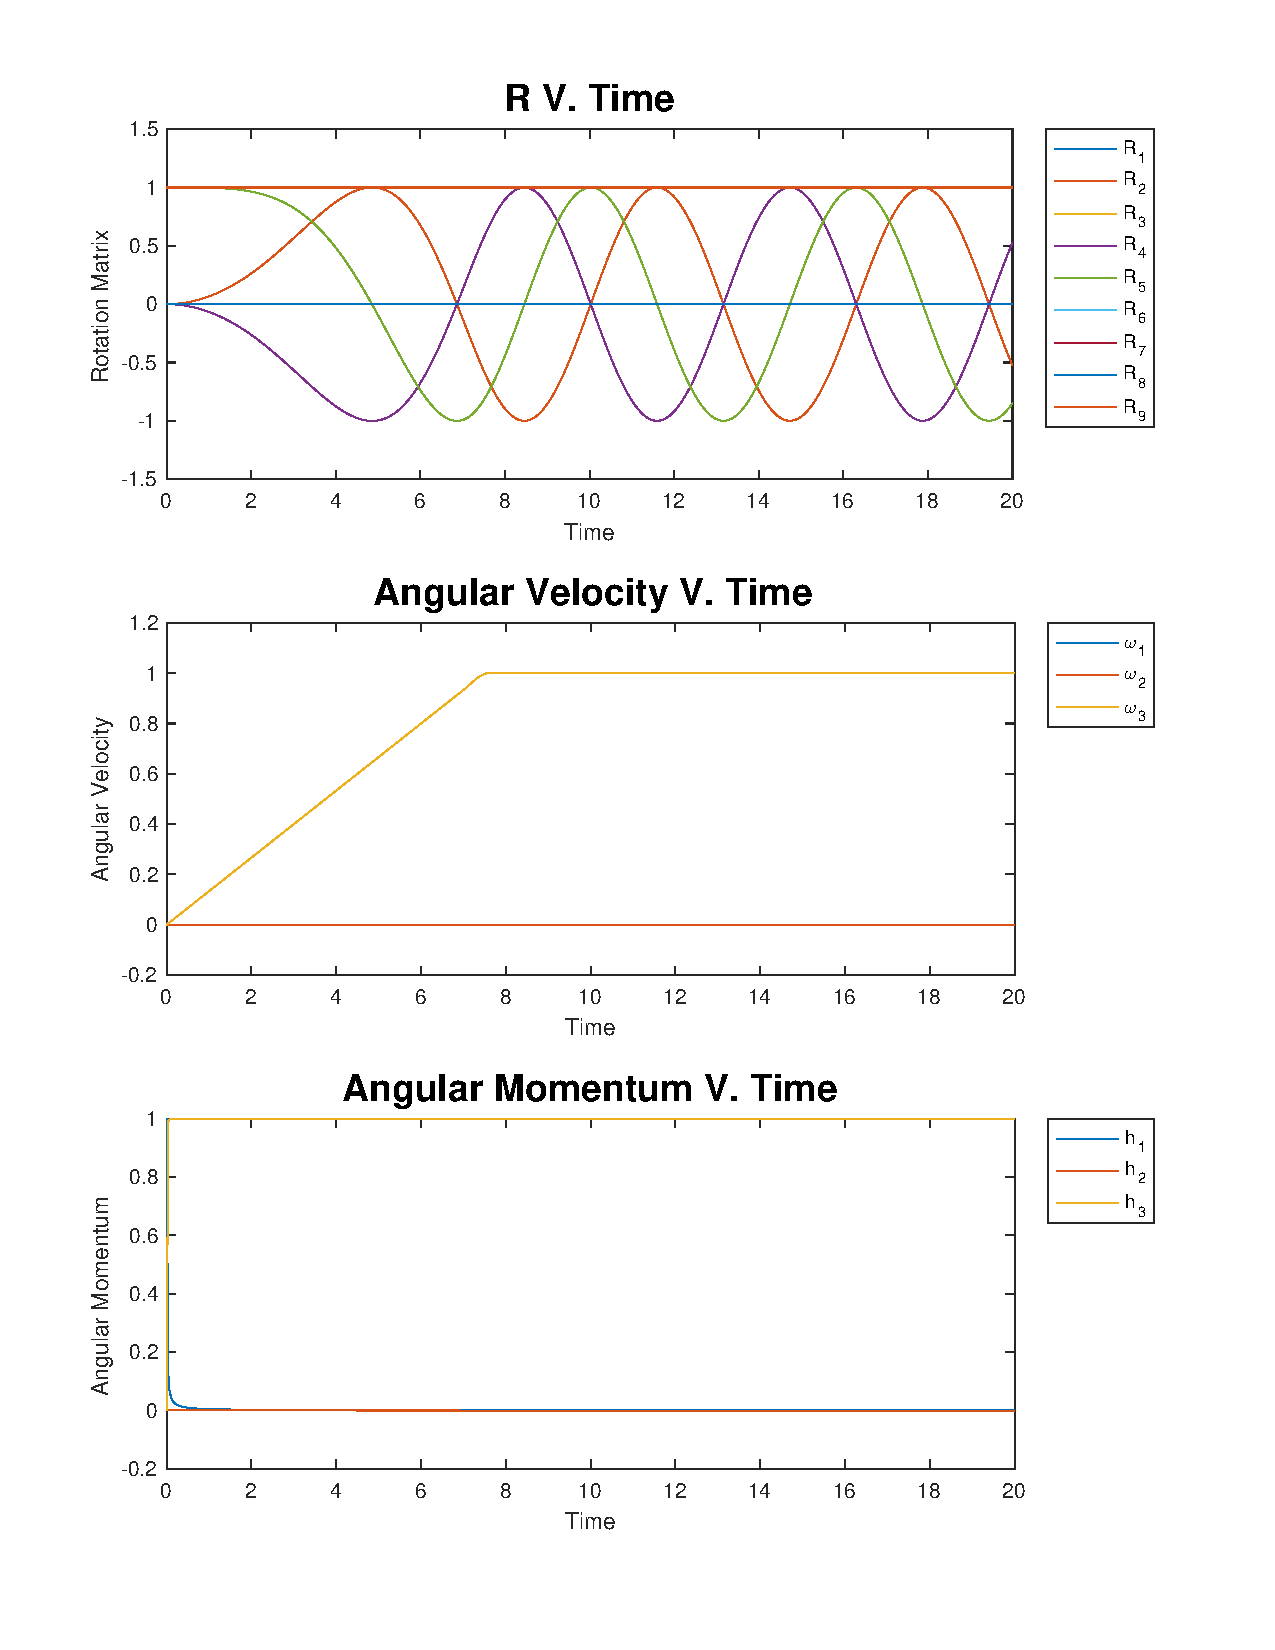
\includepdf{w0=1e-4.pdf}
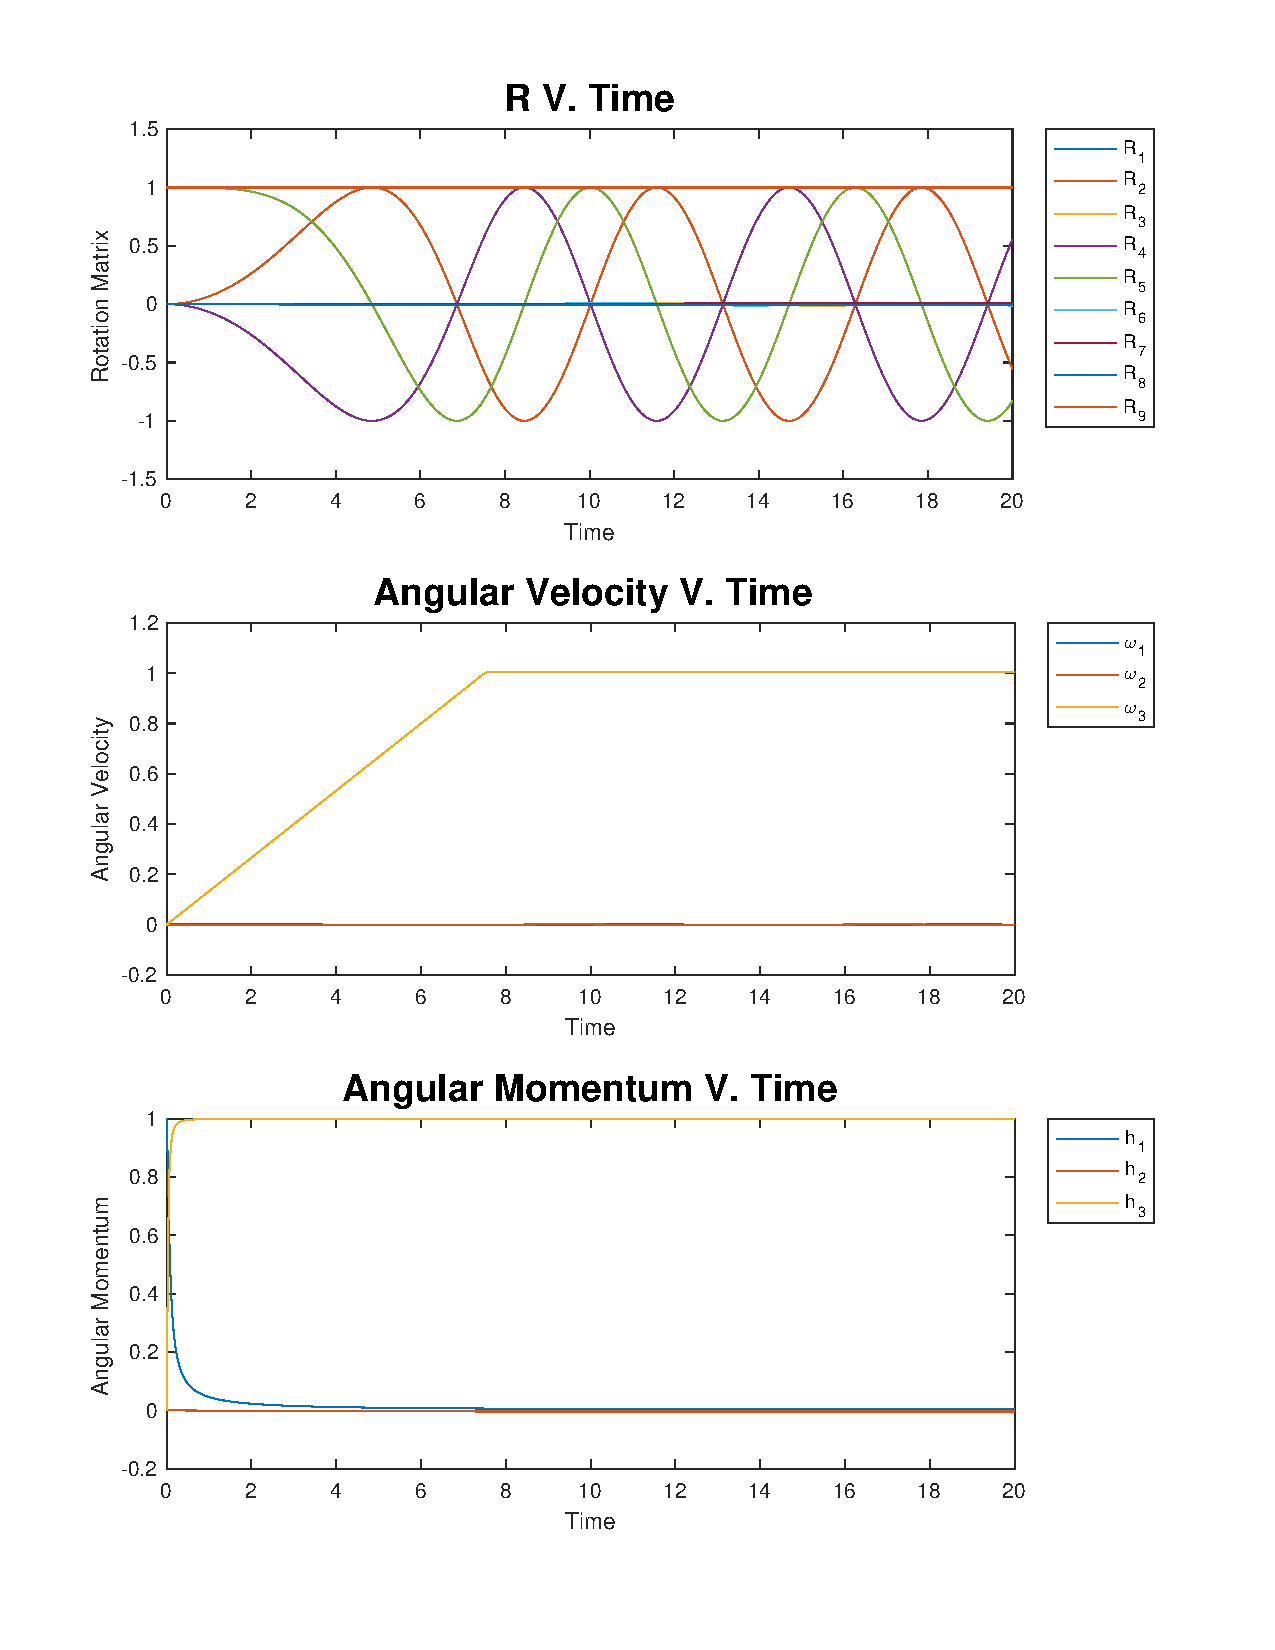
\includepdf{w0=1e-3.pdf}
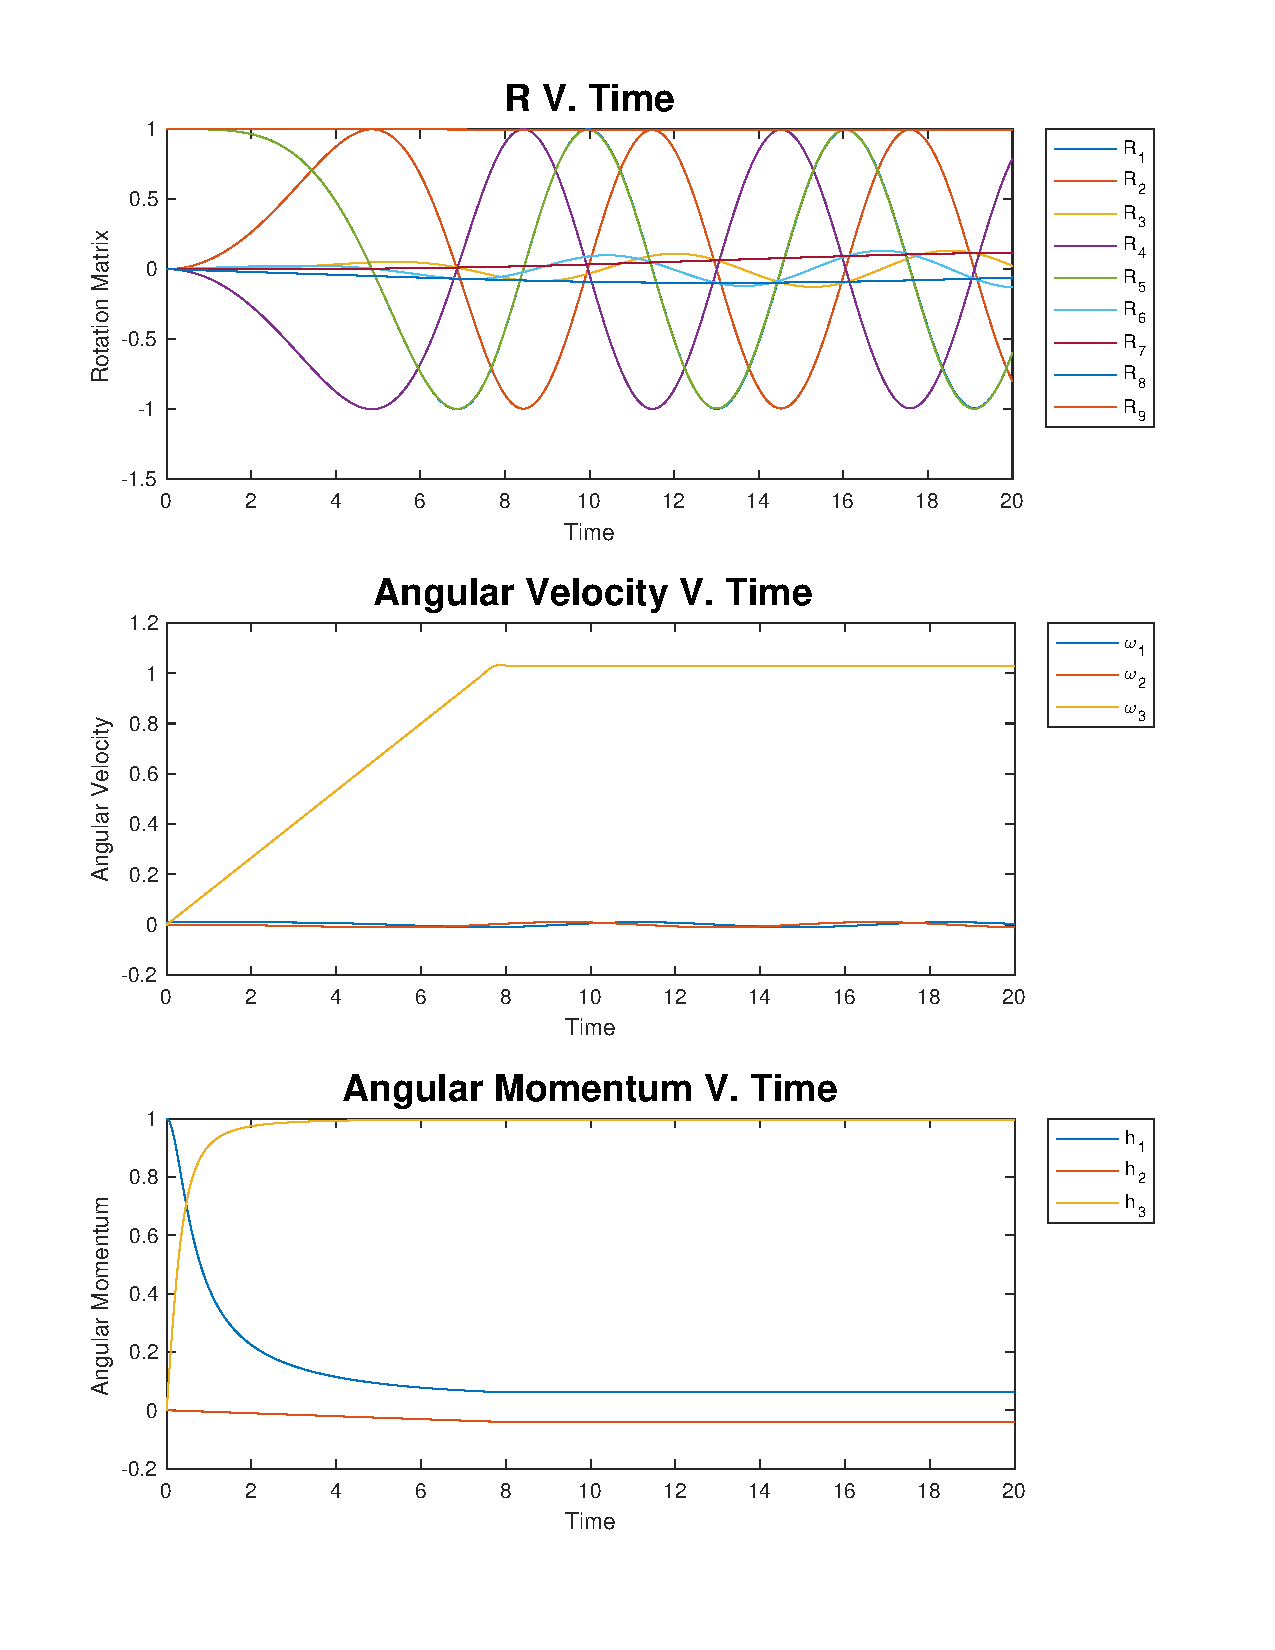
\includepdf{w0=1e-2.pdf}
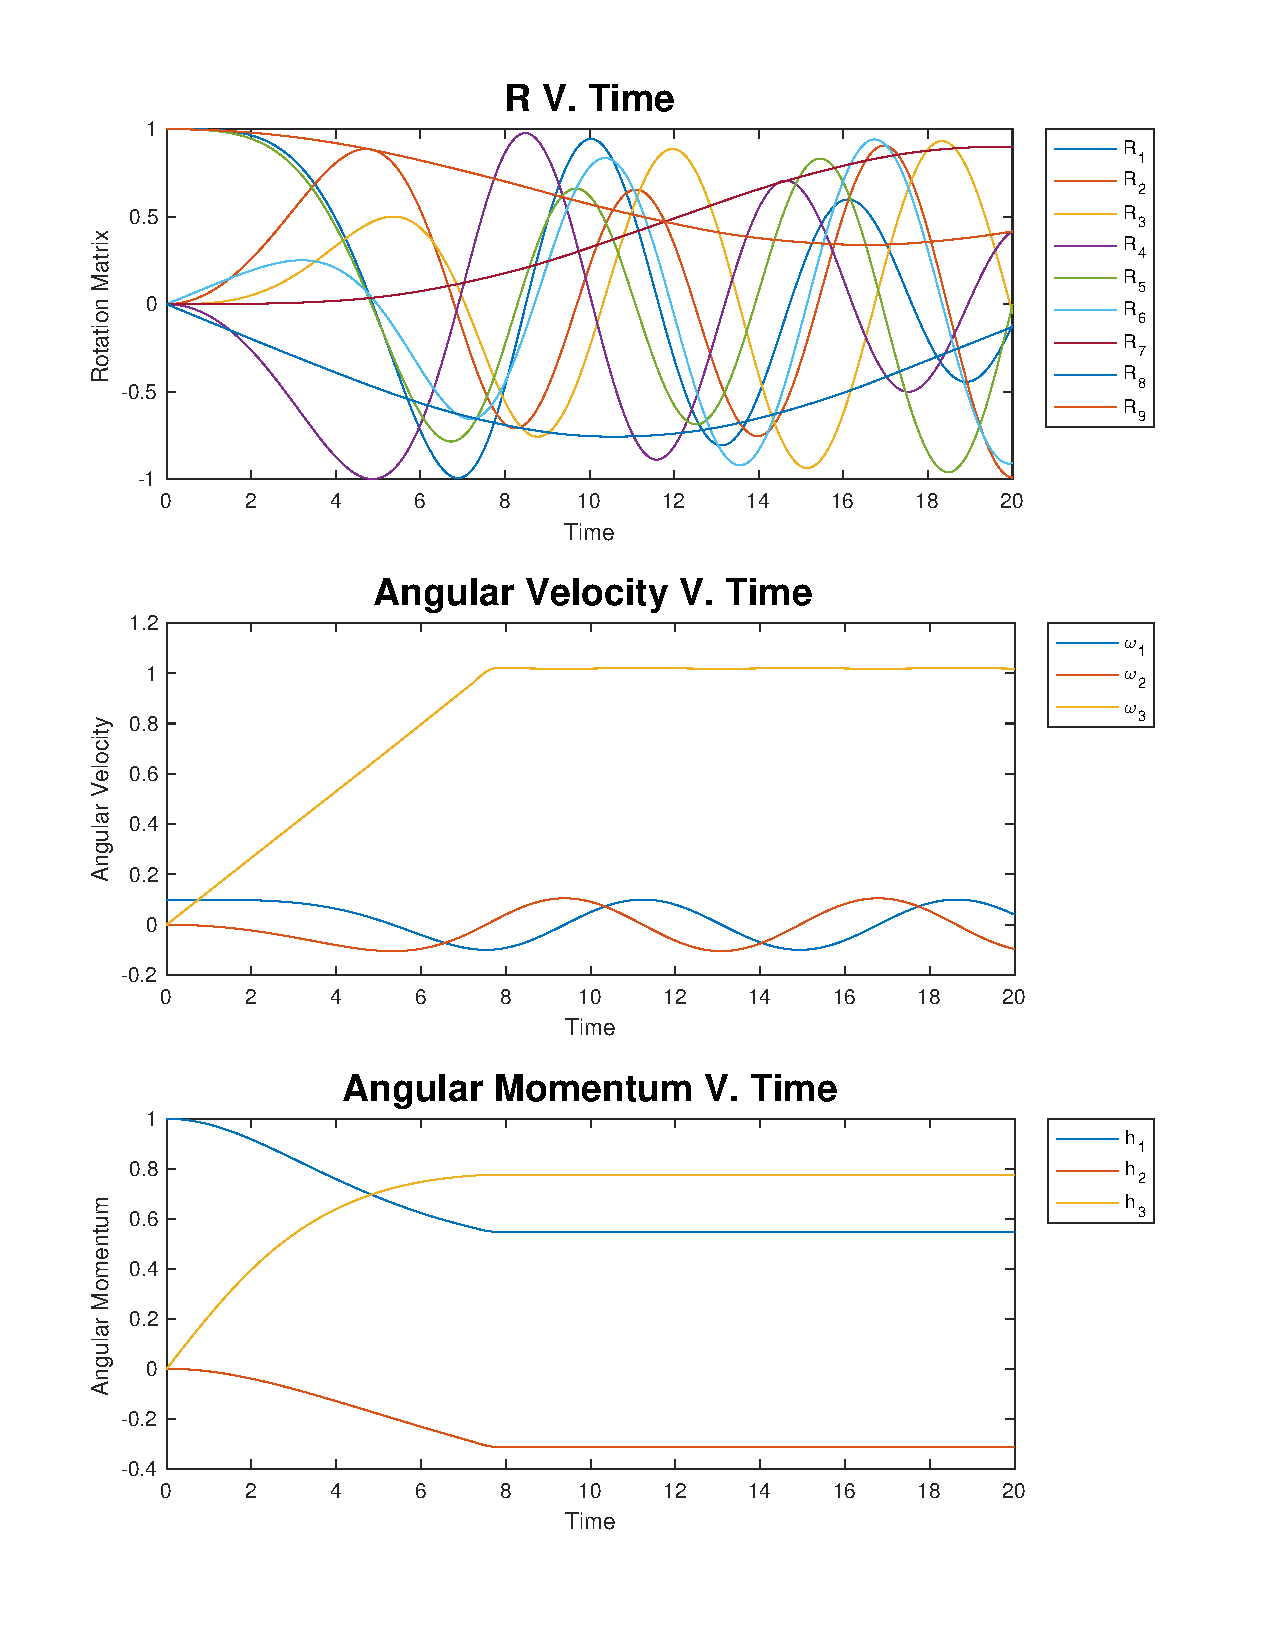
\includepdf{w0=1e-1.pdf}
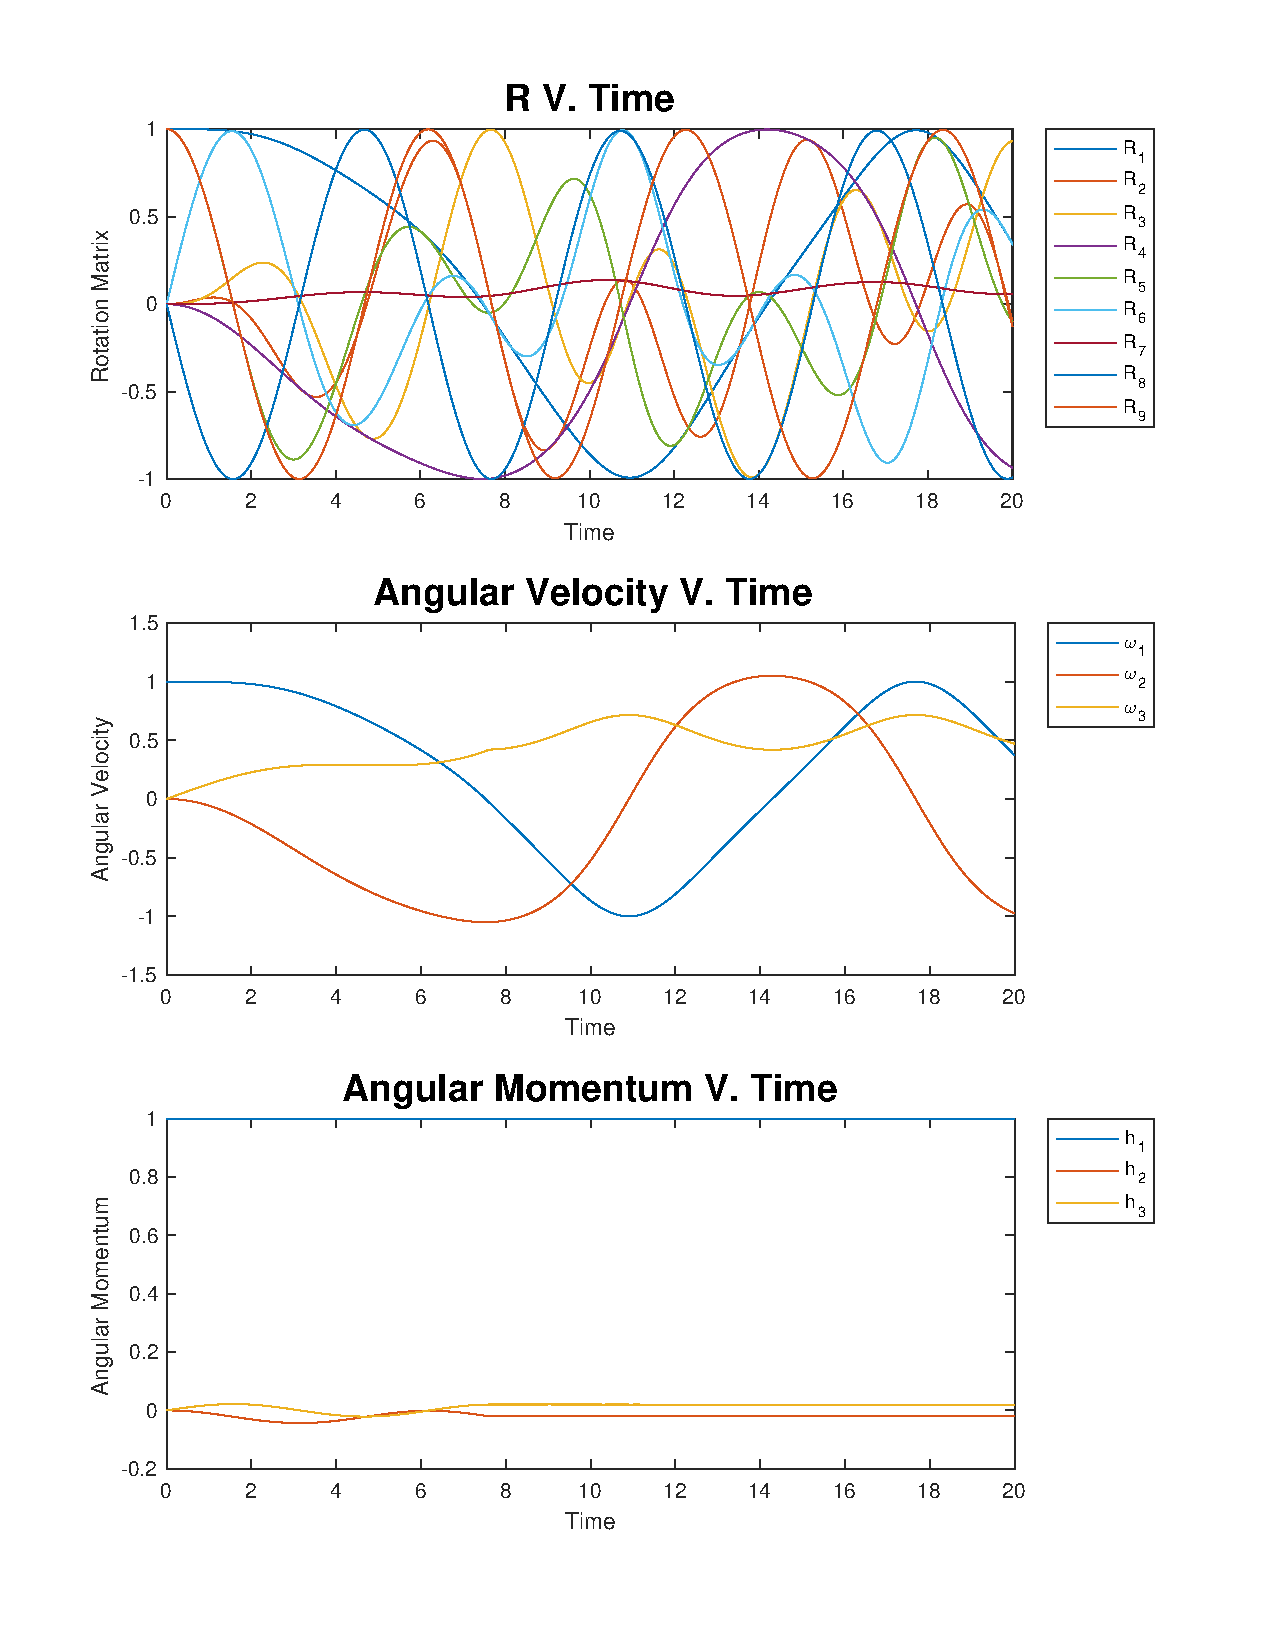
\includepdf{w0=1e0.pdf}
\end{document}